\section{Memcached}

The purpose of this chapter is to benchmark and evaluate \emph{memcached} performance. Firstly, we will examine performance under default configuration of both the server and the client. Secondly, threading will be explored in relation to latency and throughput. Finally, an execution model of multiple processes will be visited in order to establish a comparison baseline. Throughout the benchmarks, we will be focusing on latency and throughput which meets desired quality of serice.

\subsection{Default Performance}

Firstly, it is essential to establish a performance baseline of \emph{memcached} under high utilization. In order to establish the baseline, a default configuration of memcached will be used with the exception of the amount of memory allocated for exclusive use by the application. The \emph{memcached} application will be started with \lstinline! memcached -d -p 11120 -m 6144 ! specifying the port and the amount of memory to be used by the application.

In order to find out the saturation point, an increasing level of load will be applied to the client application. Therefore, a \emph{memtier} configuration with an increasing number of connections per each thread will be used. We start with 2 threads per each client and increase the number of connections each thread uses. We execute the following command to run a benchmark against the server:

\texttt{memtier\ -s\ nsl200\ -p\ 11120\ -\/-test-time=60\ -c\ \textless{}number\ of\ clients\textgreater{}\ -\/-random-data\ -\/-key-minimum=100\ -\/-key-maximum=10000}

\begin{figure}[h]
    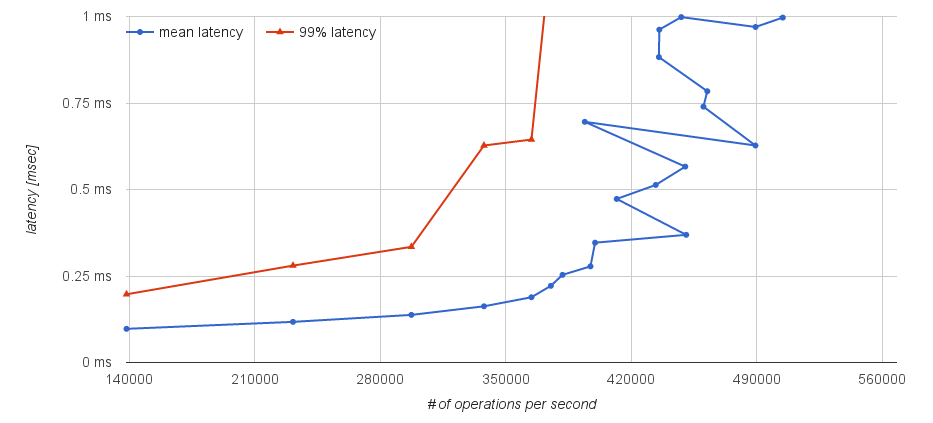
\includegraphics[width=\textwidth]{./res/5_baseline_latency_vs_ops.png}
    \caption{Throughput vs mean and 99th perecentile latency}
    \label{fig:memcached-default-latency-vs-ops}
\end{figure}

Figure \ref{fig:memcached-default-latency-vs-ops} shows the relationship between mean and 99th percentile latency against the total number of operations. We can observe that as the number of operations increases so does latency. Additionally, latency (both 99th percentile and mean) increase linearly until a saturation point is reached when a further increase in throughput is met with an exponentially larger increase in latency. The highest throughput achieved under quality of service restriction of 99th percentile latency under 1ms is 375k operations per second. The highest level of throughput corresponds to 84 simultaneous conenctions, or 12 connections per each client which is similar to benchmarks used in the literature \cite{lim2013thin}.

TODO


% \begin{figure}[h]
%     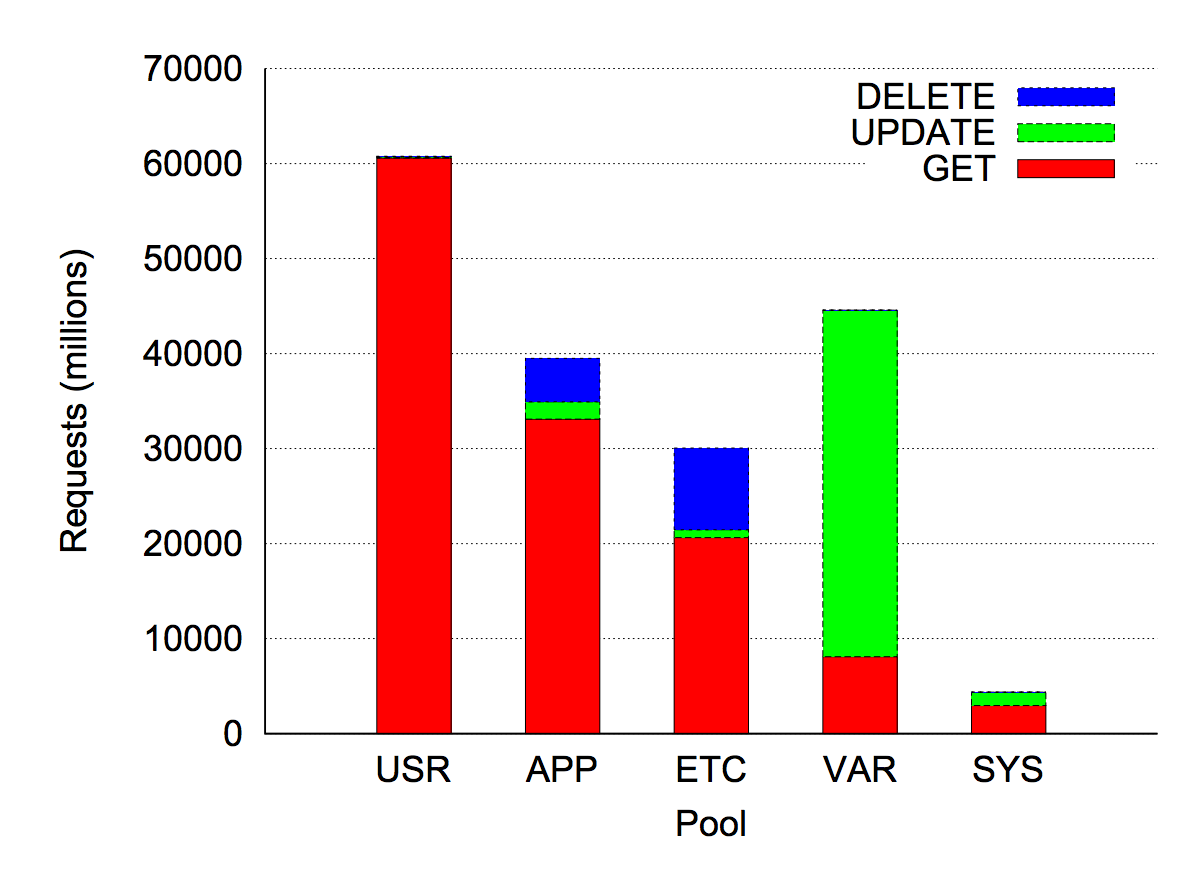
\includegraphics[width=\textwidth]{./res/5_facebook_pool_ops.png}
%     \caption{Facebook Pools Operations}
%     \label{fig:facebook-pools}
% \end{figure}


% \subsection{Throughput under QoS}
% Firstly, to establish a baseline it is essential to understand memcached behavior under high utilization. In order to establish this baseline, a default configuration of memcached will be used with a variable workload generated by the clients. Therefore, the memcached server is started with the following configuration \texttt{memcached -d -p 11120 -m 6144} setting the port and allocating 6GB of memory to memcached. Each memtier instance is configured with variable number of connections and treads such that the total number of connections (threads * number of connections per thread) is progressively increased. Memtier instances use the following configuration:
% \begin{verbatim} memtier -s nsl200 -p 11120 --test-time=60 -c (number of clients) -t (number of threads) -P memcache_binary --random-data --key-minimum=100 --key-maximum=10000 \end{verbatim}



% From the figure above, we can see that both the mean latency and the 99th perecentile latency increases linearly until we reach a saturation point at which point each increase in throughput is met with a much larger increase in latency. Additionally, we can see that the highest throughput achieved with 99th percentile under 1ms is 375k operations per second. This corresponds to 84 simultaneous connections, or 12 connections per each client. This is similar to benchmarks used in the literature [11].

% \begin{figure}[h]
%     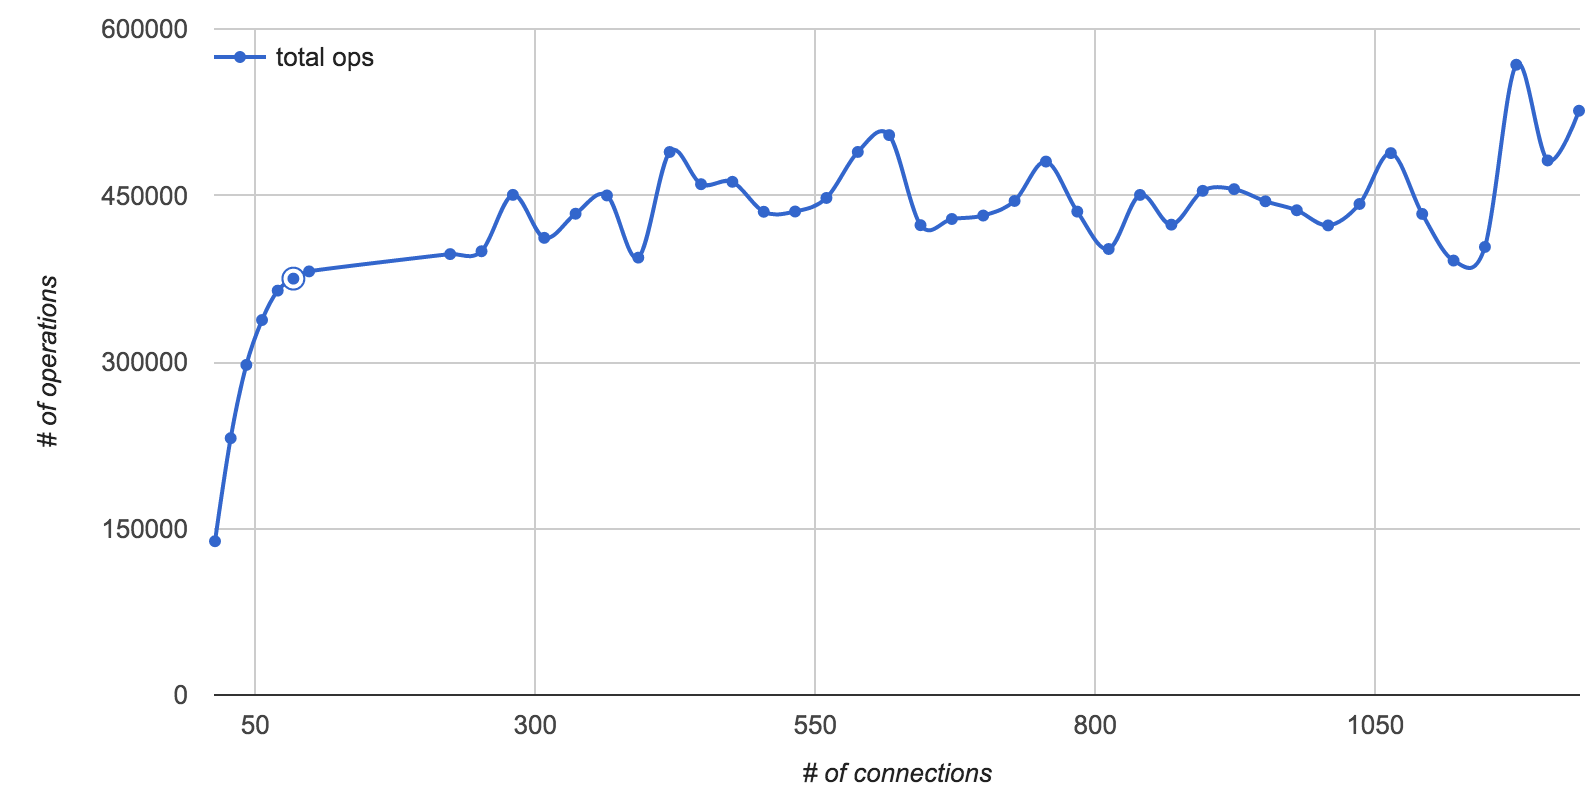
\includegraphics[width=\textwidth]{./res/5_baseline_connections_vs_ops.png}
%     \caption{Memcached Default Configuration Baseline Connections vs Ops}
%     \label{fig:memcached-default-connections-vs-ops}
% \end{figure}

% In order to further understand the impact of an increase in the number of connections, consider the figure above comparing the number of connections with the number of operations executed. We can see that memcached scales well until we reach a saturation point at around 84 connections (highlighted). A further increase in the number of connections is met with a much lower increase in the total number of operations performed. The shaded segments under the curve represent the portion of CPU time spent processing memcached (blue) and in the system (red). Furthermore, we can see that when we reach the saturation point, memcached CPU usage remains consistent while all the remaining time is spent in the system. The system requires a large number of resources to process the incoming network requests and to process the outgoing requests from memcached. Finally, the diagram also demonstrates that memcached performance is tightly linked with the performance of the network stack and the underlying hardware responsible for handling incoming and outgoing communication. This is consistent with findings in other papers [12].

\subsection{Memcached Thread Scalability}
Memcached, as a high performance object cache, is designed to be executed on a parallel architecture. It implements scalability through the use multiple threads allowing memcached to utilize many core architectures. Therefore, the next step in scaling a memcached deployment is to provision a larger number of threads for the application.

Memcached execution model is capable of processing incoming and outgoing requests in parallel, however, operations executed require a global application lock to be acquired. Therefore, the expected number of threads maximising throughput while minimizing latency can be expected to be achieved when memcached is provisioned with the same number of threads as hardware CPU cores.

Utilizing findings from the previous section, a configuration with 84 connections can be used to generate a consistent load while the number of threads provisioned for memcached can be varied. Therefore, we can set up each benchmark client as follows:
\texttt{memtier\ -s\ nsl200\ -p\ 11120\ -\/-test-time=60\ -c\ 6\ -t\ 2\ -P\ memcache_binary\ -\/-random-data\ -\/-key-minimum=100\ -\/-key-maximum=10000}
% \begin{verbatim}
% memtier -s nsl200 -p 11120
%     --test-time=30
%     -c 6
%     -t 2
%     -P memcache_binary
%     --random-data
%     --key-minimum=100 --key-maximum=10000
% \end{verbatim}

Therefore, each client is setup as follows: *memtier -s nsl200 -p 11120 --test-time=30 -c 6 -t 2 -P memcache_binary --random-data --key-minimum=100 --key-maximum=10000* and the server is configured with *memcached -d -p 11120 -m 6144 -t (threads)* where \emph{threads} varies between 1 and 35.

% \begin{figure}[h]
%     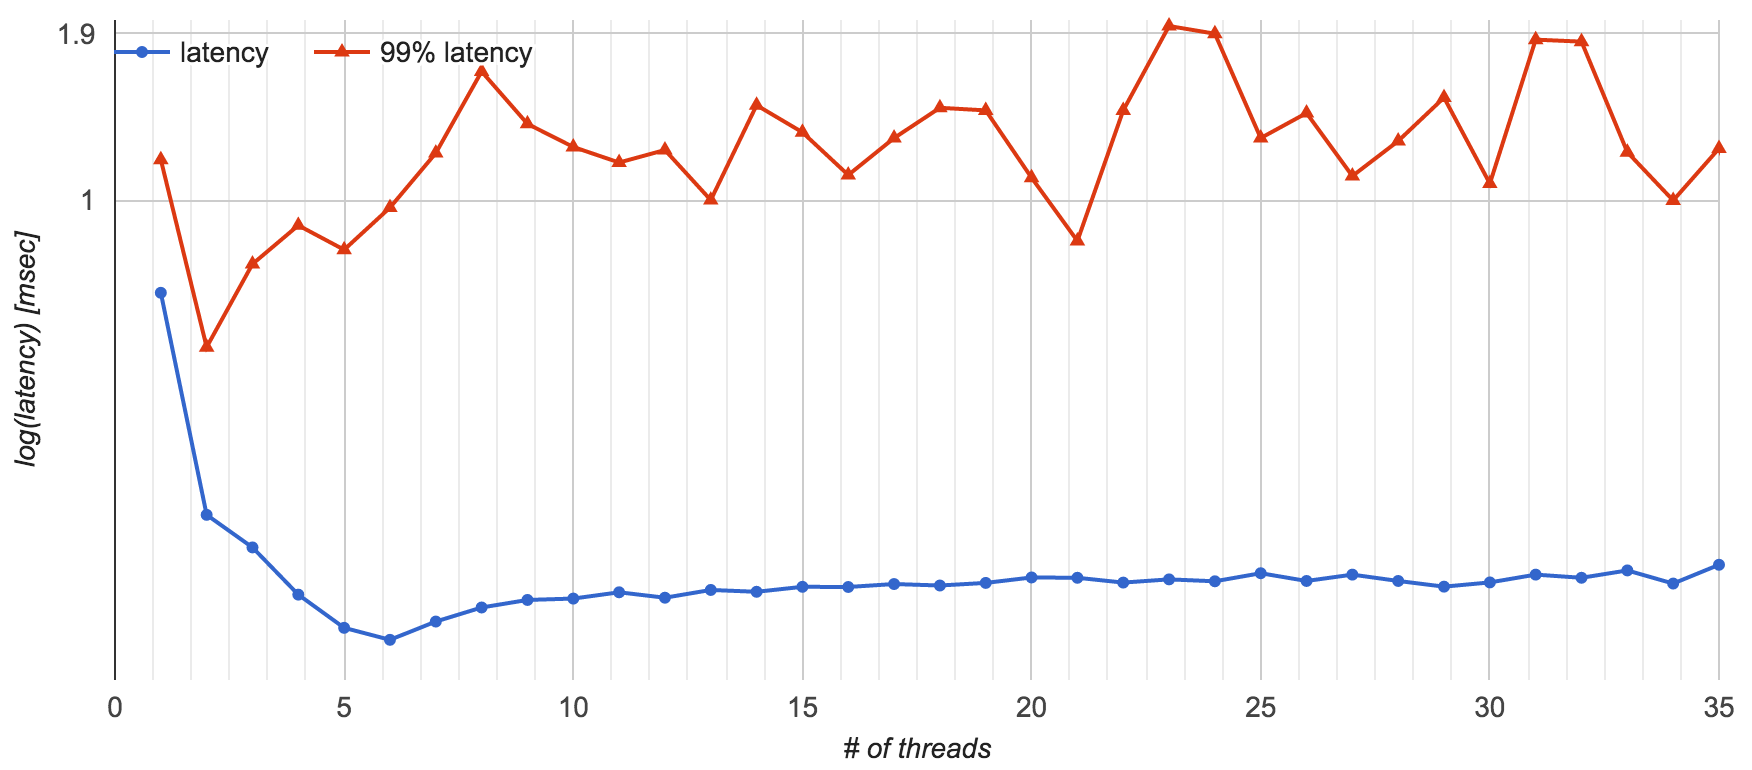
\includegraphics[width=\textwidth]{./res/5_threads_latency.png}
%     \caption{Memcached Thread Scaling}
%     \label{fig:memcached-threads}
% \end{figure}

% The figure above shows mean and 99th percentile latency against the number of threads. The lowest mean latency occurs when running 6 threads of memcached. This corresponds to the expectation of best performance of using *n* threads with *n* CPU cores. Additionally, less than 6 threads exhibits higher latency than when using 6 cores. A constant load created against the server and the number of threads less than the number of CPUs creates a bottleneck where network requests targeted for a given core are attempted to be processed only by a given core to avoid an expensive data transfer and a context switch. Consequently, the queue of requests builds up and overall latency decreases. An increase in the number of threads allows for a higher throughput due to reduced bottleneck on request processing. Furthermore, latency increases with the number of threads as a context switch is required between contexts in each thread therefore putting additional strain on the operating system resources.

% The 99th percentile lantecy behaves similarly to the mean latency. We can observe that 99th precentile latency drops below the defined quality of service when using between 2 and 6 threads. Beyond six threads, 99th percentile behavior fluctuates above the desired quality of service boundary.

% \begin{figure}[h]
%     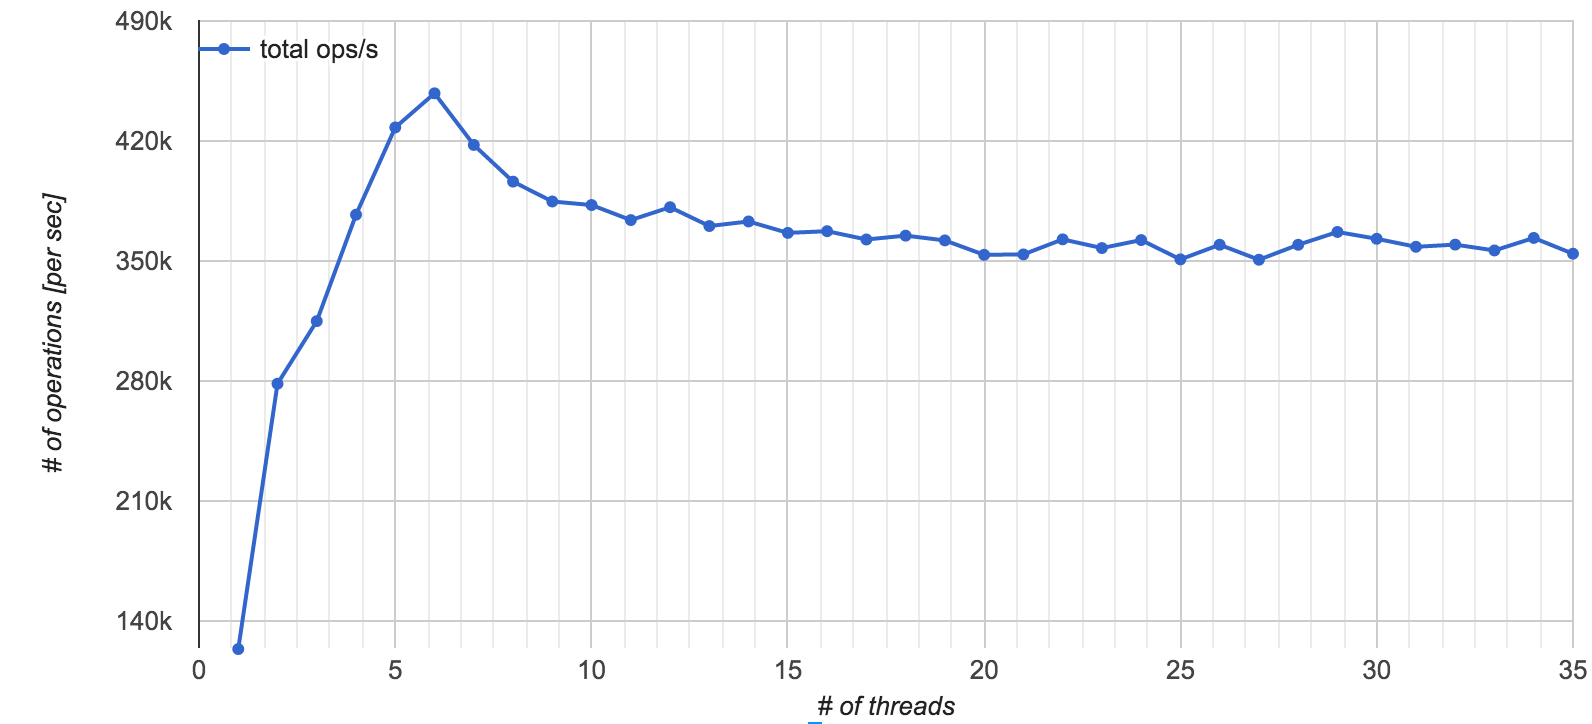
\includegraphics[width=\textwidth]{./res/5_threads_total_ops.png}
%     \caption{Memcached Thread Total Ops}
%     \label{fig:memcached-threads-total-ops}
% \end{figure}

% Similarly to latency behavior, throughput is the highest when when running 6 threads - close to 450k operations per second. This is in accordance with our expectation as resources are being utilized fully and overhead from context switching is limited. Additionally, we can see that throughput incrases drastically between 1 and 6 threads, that is, from 120k to 450k. A further increase in the number of threads beyond 6 threads only results in a reduction in overall throughput caused by context switching overheads and operating system resource requirements.

% \begin{figure}[h]
%     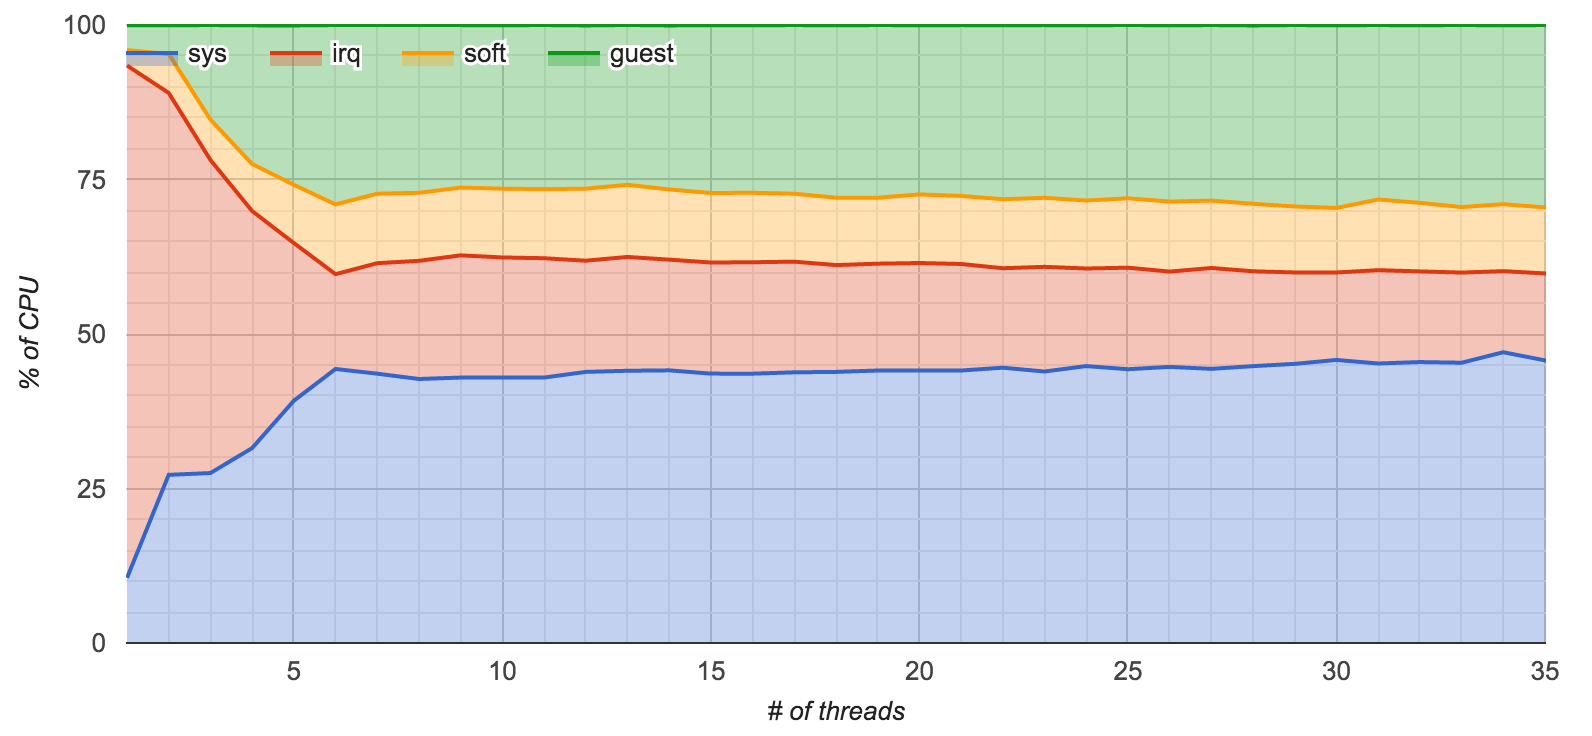
\includegraphics[width=\textwidth]{./res/5_threads_cpu.png}
%     \caption{Memcached Thread CPU}
%     \label{fig:memcached-threads-cpu}
% \end{figure}

% Analysing the CPU usage as we increase the number of threads, we can observe that initially a large portion of the CPU time is spent servicing hardware interrupts (*irq*). Therefore, the OS is handling incoming traffic interrupts from the NIC. As the number of threads increases, an increasingly larger portion of CPU time is spent processing system calls and context switching (*sys*). This is reasonable as a larger number of threads will require context switching and concurrency management provided by the operating system. We can see that time spent processing hardware interrupts (*irq*) decreases which has the effect of increasing latency as packets remained queued up in the NIC for longer before the OS manages to schedule the interrupt to be serviced. Furthermore, we can observe that software iterrupts (*soft*) CPU time progressively increases until we reach 6 threads and remains stable as the number of threads grows further. The initial increase is reasonable as we are demanding more threads to processed simultanesly, past this point the percentage remains stable as we have reached a saturation point in terms of scalability and server performance. Finally, memcached (*guest*) follows a similar pattern as software interrupts. Usage increases until 6 threads are used and saturates further. This is further indicative of the inability to efficiently scale the number of threads past the point at which memcached uses the same number of threads as CPU cores.

% \subsection{Thread pinning}
% Thread pinning is the process of assigning a \emph{set_irq_affinity} to each individual thread. As suggested by Leverich and Kozyrakis, "pinning memcached threads to distinct cores greatly improves load balance, consequently improving tail latency." [13] and therefore the reasonable next step in optimizing memcached performance is to attempt thread pinning and analyse the results obtained.

% By default, when a new process is started, its affinity is set to all available CPUs. We can discover a given process affinity by executing \verb{taskset -p (pid) } where \verb{pid} is the process identifier.

% "A Memcache instance started with n threads will spawn n + 1 threads of which the first n are worker threads and the last is a maintenance thread used for hash table expansion under high load factor." [14]. We can discover memcached threads used for request processing using
% \verb{ps -p (memcache-process-id) -o tid= -L | sort -n | tail -n +2 | head -n -1} [14] and further set their processor affinity using \verb{taskset -pc (cpu-id) (tid)} where *tid* is the thread id discovered previously [14].

% Given the best performance under QoS constraints of 1ms found in the previous section is memcached with 6 threads, the following benchmark will be using this best configuration in order the analyze the impact of thread pinning.

% \begin{figure}[h]
%     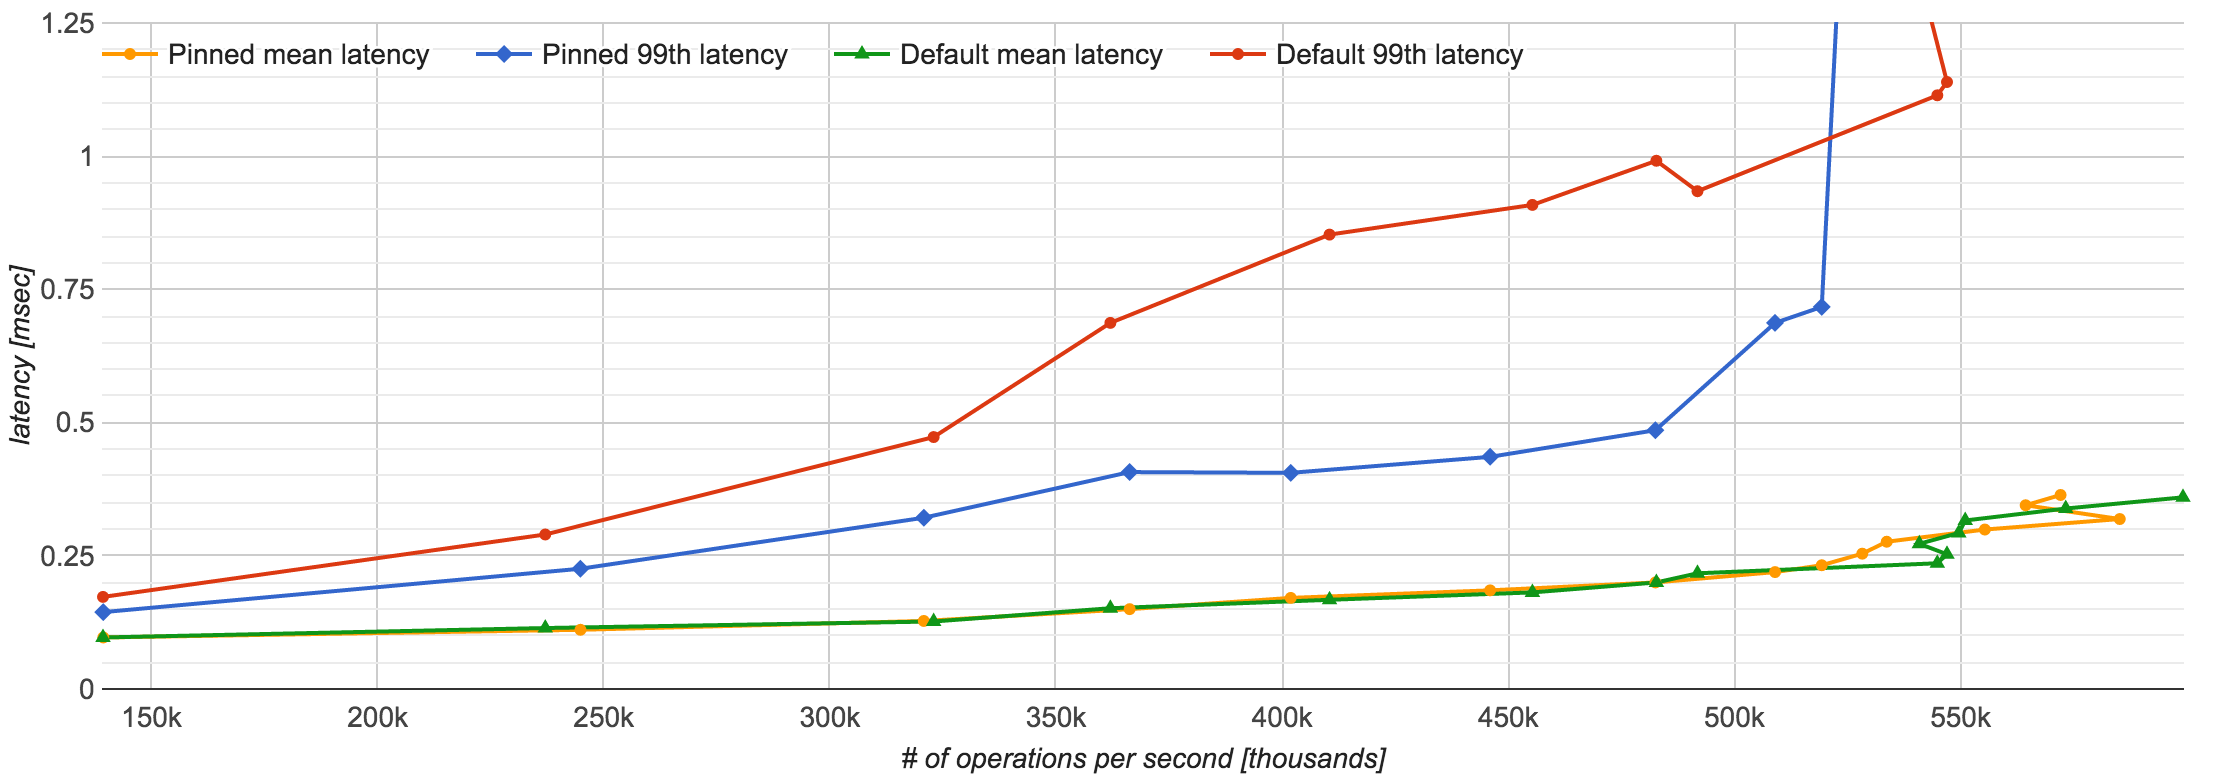
\includegraphics[width=\textwidth]{./res/5_threads_pinned_vs_default.png}
%     \caption{Memcached Pinned Threads vs Unpinned}
%     \label{fig:memcached-threads-pinned-vs-default}
% \end{figure}


% % % % * [1] [memcached.org](http://memcached.org/)
% % % % * [2] An FPGA-based in-line accelerator for Memcached, Maysam Lavasani, Hari Angepat, and Derek Chiou
% % % % * [3] [New Commands, Memcached.org](https://code.google.com/p/memcached/wiki/NewCommands)
% % % % * [4] [Scaling memcached at Facebook](https://www.facebook.com/notes/facebook-engineering/scaling-memcached-at-facebook/39391378919/)
% % % % * [5]
% % % % * [6] [Amazon ElastiCache](http://aws.amazon.com/elasticache/)
% % % % * [7] Workload Analysis of a Large-Scale Key-Value Store, Berk Atikoglu, Yuehai Xu, Eitan Frachtenberg, Song Jiang, Mike Paleczny
% % % % * [8] http://investor.fb.com/releasedetail.cfm?ReleaseID=908022
% % % % * [9] [Twemproxy](https://github.com/twitter/twemproxy)
% % % % * [10] [Enhancing the Scalability of Memcached](https://software.intel.com/sites/default/files/m/0/b/6/1/d/45675-memcached_05172012.pdf)
% % % % * [11] Thin Servers with Smart Pipes: Designing SoC Accelerators for Memcached - Kevin Lim, David Meisner, Ali G. Saidi, Parthasarathy Ranganathan, Thomas F. Wenisch
% % % % * [12] MICA: A Holistic Approach to Fast In-Memory Key-Value Storage
% % % % * [13] Reconciling High Server Utilization and Sub-millisecond Quality-of-Service, Jacob Leverich Christos Kozyrakis
% % % % * [14] Filling The Pipe: A Guide To Optimising Memcache Performance On Solarflare Hardware